\section{Pregunta \texttt{f)}}\label{pregunta-f}

A continuación, nos interesa determinar un equivalente discreto para el
sistema, considerando un tiempo de muestreo $T_{m} = 200\ \unit{ms}$.

Para esto, vamos a utilizar las matrices del sistema que obtuvimos en la pregunta
\hyperref[pregunta-b]{\texttt{b)}}:
\begin{align}
    \pmb{A} &= \begin{bmatrix}
        0 & 1 & 0 \\
        -\frac{\nara{a_{0\psi}}}{\nara{a_{2\psi}}}   & -\frac{\nara{a_{1\psi}}}{\nara{a_{2\psi}}} & \frac{\nara{b_{0\psi}}}{\nara{a_{2\psi}}} - \frac{\nara{b_{1\psi}}\nara{a_{0\omega}}}{\nara{a_{2\psi}}\nara{a_{1\omega}}} \\
        0 & 0 & -\frac{\nara{a_{0\omega}}}{\nara{a_{1\omega}}}
    \end{bmatrix} &
    \pmb{B} &= \begin{bmatrix}
        0 \\
        \frac{\nara{b_{1\psi}}\nara{b_{0\omega}}}{\nara{a_{2\psi}}\nara{a_{1\omega}}} \\
        \frac{\nara{b_{0\omega}}}{\nara{a_{1\omega}}}
    \end{bmatrix}
\end{align}
\begin{align}
  \pmb{C} &= \begin{bmatrix}
    1 & 0 & 0
  \end{bmatrix}
\end{align}

De lo visto en el curso de Sistemas Lineales Dinámicos \cite{apunte-sld}, sabemos
que para obtener el equivalente discreto de estas matrices debemos realizar los
siguientes cálculos:
\begin{equation}
    \mathbf{A_d}= e^{\mathbf{A}T_{m}} ,\quad \mathbf{B_d}= \int_{0}^{T_{m}} e^{\mathbf{A}(T_{m}-\sigma)}\mathbf{B}  \,d\sigma 
\end{equation}

Nos ayudamos entonces de \textit{MATLAB} para determinar los valores de estas
matrices, y obtenemos:
\begin{align}
    \mathbf{A_d} &= \begin{bmatrix}
        -0.1106 & 0.0970 & 0.7400 \\
        -7.6484 &  -0.2385 & 4.5822 \\
        0 & 0 & 0.7386
    \end{bmatrix} &
    \mathbf{B_d} &= \begin{bmatrix}
        0.0090 \\
        0.0710 \\
        0.0046
    \end{bmatrix}
\end{align}

Además, como la salida del sistema es $\rojo{\psi}$, y no hay perturbaciones,
se tiene que las matrices $\pmb{C_{d}}$ y $\pmb{D_{d}}$ son:
\begin{align}
  \pmb{C_{d}} &= \begin{bmatrix}
      1 & 0 & 0
  \end{bmatrix} &
  \pmb{D_{d}} &= 0
\end{align}

Luego, calculamos los valores propios del sistema. Para esto, se utilizón el
comando \verb|eig| de \textit{MATLAB}, entonces:
\begin{align}
  \lambda_{0} &=  0.7386 \\
  \lambda_{1,2} &=  -0.1745 \pm 0.8588j
\end{align}

A continuación, simularemos el sistema para una entrada
$\verd{v_{i}}(kT) = \frac{\verd{v_{i0}}}{3}\left(r(kT-1) - r(kT-4)\right)$
y un tiempo $0 \leq kT \leq 10\ \unit{s}$, y graficaremos los valores que
toman las variables de estado para esta entrada. Nuevamente nos ayudamos
de \textit{MATLAB}, pero esta vez se utilizó el comando \verb|ss2tf| para
obtener una representación en función de transferencia discreta del sistema,
para luego, con el comando \verb|filter| simular el sistema para la entrada
dada. Además, a diferencia del caso continuo, se utilizó el comando \verb|stem|
en lugar de \verb|plot| para graficar.

El código para realizar los cálculos, simular el sistema y luego graficar está
disponible en el \autoref{lst:problema-f}.

\begin{figure}[h]
  \centering
  % This file was created by matlab2tikz.
%
%The latest updates can be retrieved from
%  http://www.mathworks.com/matlabcentral/fileexchange/22022-matlab2tikz-matlab2tikz
%where you can also make suggestions and rate matlab2tikz.
%
\begin{tikzpicture}

\begin{axis}[%
width=0.856\textwidth,
height=0.159\textheight,
at={(0\textwidth,0.491\textheight)},
scale only axis,
xmin=-0.2,
xmax=10.2,
xlabel style={font=\color{white!15!black}},
xlabel={Tiempo $[\unit{s}]$},
ymin=-1,
ymax=28,
ylabel style={font=\color{white!15!black}},
ylabel={$\verd{v_{i}}(t)\ [\unit{V}]$},
axis background/.style={fill=white},
title style={font=\bfseries},
title={Voltaje del motor}
]
\addplot[ycomb, color=Green, mark=*, mark options={solid, Green}, forget plot] table[row sep=crcr] {%
0	0\\
0.2	0\\
0.4	0\\
0.6	0\\
0.8	0\\
1	0\\
1.2	1.76637280517777\\
1.4	3.53274561035553\\
1.6	5.29911841553329\\
1.8	7.06549122071106\\
2	8.83186402588882\\
2.2	10.5982368310666\\
2.4	12.3646096362444\\
2.6	14.1309824414221\\
2.8	15.8973552465999\\
3	17.6637280517776\\
3.2	19.4301008569554\\
3.4	21.1964736621332\\
3.6	22.9628464673109\\
3.8	24.7292192724887\\
4	26.4955920776665\\
4.2	26.4955920776665\\
4.4	26.4955920776665\\
4.6	26.4955920776665\\
4.8	26.4955920776665\\
5	26.4955920776665\\
5.2	26.4955920776665\\
5.4	26.4955920776665\\
5.6	26.4955920776665\\
5.8	26.4955920776665\\
6	26.4955920776665\\
6.2	26.4955920776665\\
6.4	26.4955920776665\\
6.6	26.4955920776665\\
6.8	26.4955920776665\\
7	26.4955920776665\\
7.2	26.4955920776665\\
7.4	26.4955920776665\\
7.6	26.4955920776665\\
7.8	26.4955920776665\\
8	26.4955920776665\\
8.2	26.4955920776665\\
8.4	26.4955920776665\\
8.6	26.4955920776665\\
8.8	26.4955920776665\\
9	26.4955920776665\\
9.2	26.4955920776665\\
9.4	26.4955920776665\\
9.6	26.4955920776665\\
9.8	26.4955920776665\\
10	26.4955920776665\\
};
\addplot [color=Green, forget plot]
  table[row sep=crcr]{%
0	0\\
0.01	0\\
0.02	0\\
0.03	0\\
0.04	0\\
0.05	0\\
0.06	0\\
0.07	0\\
0.08	0\\
0.09	0\\
0.1	0\\
0.11	0\\
0.12	0\\
0.13	0\\
0.14	0\\
0.15	0\\
0.16	0\\
0.17	0\\
0.18	0\\
0.19	0\\
0.2	0\\
0.21	0\\
0.22	0\\
0.23	0\\
0.24	0\\
0.25	0\\
0.26	0\\
0.27	0\\
0.28	0\\
0.29	0\\
0.3	0\\
0.31	0\\
0.32	0\\
0.33	0\\
0.34	0\\
0.35	0\\
0.36	0\\
0.37	0\\
0.38	0\\
0.39	0\\
0.4	0\\
0.41	0\\
0.42	0\\
0.43	0\\
0.44	0\\
0.45	0\\
0.46	0\\
0.47	0\\
0.48	0\\
0.49	0\\
0.5	0\\
0.51	0\\
0.52	0\\
0.53	0\\
0.54	0\\
0.55	0\\
0.56	0\\
0.57	0\\
0.58	0\\
0.59	0\\
0.6	0\\
0.61	0\\
0.62	0\\
0.63	0\\
0.64	0\\
0.65	0\\
0.66	0\\
0.67	0\\
0.68	0\\
0.69	0\\
0.7	0\\
0.71	0\\
0.72	0\\
0.73	0\\
0.74	0\\
0.75	0\\
0.76	0\\
0.77	0\\
0.78	0\\
0.79	0\\
0.8	0\\
0.81	0\\
0.82	0\\
0.83	0\\
0.84	0\\
0.85	0\\
0.86	0\\
0.87	0\\
0.88	0\\
0.89	0\\
0.9	0\\
0.91	0\\
0.92	0\\
0.93	0\\
0.94	0\\
0.95	0\\
0.96	0\\
0.97	0\\
0.98	0\\
0.99	0\\
1	0\\
1.01	0.0883186402588882\\
1.02	0.176637280517776\\
1.03	0.264955920776665\\
1.04	0.353274561035553\\
1.05	0.441593201294441\\
1.06	0.529911841553329\\
1.07	0.618230481812217\\
1.08	0.706549122071106\\
1.09	0.794867762329994\\
1.1	0.883186402588882\\
1.11	0.97150504284777\\
1.12	1.05982368310666\\
1.13	1.14814232336555\\
1.14	1.23646096362443\\
1.15	1.32477960388332\\
1.16	1.41309824414221\\
1.17	1.5014168844011\\
1.18	1.58973552465999\\
1.19	1.67805416491887\\
1.2	1.76637280517776\\
1.21	1.85469144543665\\
1.22	1.94301008569554\\
1.23	2.03132872595443\\
1.24	2.11964736621331\\
1.25	2.2079660064722\\
1.26	2.29628464673109\\
1.27	2.38460328698998\\
1.28	2.47292192724887\\
1.29	2.56124056750776\\
1.3	2.64955920776664\\
1.31	2.73787784802553\\
1.32	2.82619648828442\\
1.33	2.91451512854331\\
1.34	3.0028337688022\\
1.35	3.09115240906108\\
1.36	3.17947104931997\\
1.37	3.26778968957886\\
1.38	3.35610832983775\\
1.39	3.44442697009664\\
1.4	3.53274561035553\\
1.41	3.62106425061441\\
1.42	3.7093828908733\\
1.43	3.79770153113219\\
1.44	3.88602017139108\\
1.45	3.97433881164996\\
1.46	4.06265745190885\\
1.47	4.15097609216774\\
1.48	4.23929473242663\\
1.49	4.32761337268552\\
1.5	4.41593201294441\\
1.51	4.50425065320329\\
1.52	4.59256929346218\\
1.53	4.68088793372107\\
1.54	4.76920657397996\\
1.55	4.85752521423885\\
1.56	4.94584385449773\\
1.57	5.03416249475662\\
1.58	5.12248113501551\\
1.59	5.2107997752744\\
1.6	5.29911841553329\\
1.61	5.38743705579218\\
1.62	5.47575569605106\\
1.63	5.56407433630995\\
1.64	5.65239297656884\\
1.65	5.74071161682773\\
1.66	5.82903025708662\\
1.67	5.9173488973455\\
1.68	6.00566753760439\\
1.69	6.09398617786328\\
1.7	6.18230481812217\\
1.71	6.27062345838106\\
1.72	6.35894209863994\\
1.73	6.44726073889883\\
1.74	6.53557937915772\\
1.75	6.62389801941661\\
1.76	6.7122166596755\\
1.77	6.80053529993438\\
1.78	6.88885394019327\\
1.79	6.97717258045216\\
1.8	7.06549122071105\\
1.81	7.15380986096994\\
1.82	7.24212850122883\\
1.83	7.33044714148771\\
1.84	7.4187657817466\\
1.85	7.50708442200549\\
1.86	7.59540306226438\\
1.87	7.68372170252327\\
1.88	7.77204034278216\\
1.89	7.86035898304104\\
1.9	7.94867762329993\\
1.91	8.03699626355882\\
1.92	8.1253149038177\\
1.93	8.21363354407659\\
1.94	8.30195218433548\\
1.95	8.39027082459437\\
1.96	8.47858946485326\\
1.97	8.56690810511215\\
1.98	8.65522674537103\\
1.99	8.74354538562992\\
2	8.83186402588881\\
2.01	8.9201826661477\\
2.02	9.00850130640659\\
2.03	9.09681994666548\\
2.04	9.18513858692436\\
2.05	9.27345722718325\\
2.06	9.36177586744214\\
2.07	9.45009450770103\\
2.08	9.53841314795992\\
2.09	9.6267317882188\\
2.1	9.71505042847769\\
2.11	9.80336906873658\\
2.12	9.89168770899547\\
2.13	9.98000634925435\\
2.14	10.0683249895132\\
2.15	10.1566436297721\\
2.16	10.244962270031\\
2.17	10.3332809102899\\
2.18	10.4215995505488\\
2.19	10.5099181908077\\
2.2	10.5982368310666\\
2.21	10.6865554713255\\
2.22	10.7748741115844\\
2.23	10.8631927518432\\
2.24	10.9515113921021\\
2.25	11.039830032361\\
2.26	11.1281486726199\\
2.27	11.2164673128788\\
2.28	11.3047859531377\\
2.29	11.3931045933966\\
2.3	11.4814232336555\\
2.31	11.5697418739143\\
2.32	11.6580605141732\\
2.33	11.7463791544321\\
2.34	11.834697794691\\
2.35	11.9230164349499\\
2.36	12.0113350752088\\
2.37	12.0996537154677\\
2.38	12.1879723557266\\
2.39	12.2762909959854\\
2.4	12.3646096362443\\
2.41	12.4529282765032\\
2.42	12.5412469167621\\
2.43	12.629565557021\\
2.44	12.7178841972799\\
2.45	12.8062028375388\\
2.46	12.8945214777977\\
2.47	12.9828401180566\\
2.48	13.0711587583154\\
2.49	13.1594773985743\\
2.5	13.2477960388332\\
2.51	13.3361146790921\\
2.52	13.424433319351\\
2.53	13.5127519596099\\
2.54	13.6010705998688\\
2.55	13.6893892401277\\
2.56	13.7777078803865\\
2.57	13.8660265206454\\
2.58	13.9543451609043\\
2.59	14.0426638011632\\
2.6	14.1309824414221\\
2.61	14.219301081681\\
2.62	14.3076197219399\\
2.63	14.3959383621988\\
2.64	14.4842570024577\\
2.65	14.5725756427165\\
2.66	14.6608942829754\\
2.67	14.7492129232343\\
2.68	14.8375315634932\\
2.69	14.9258502037521\\
2.7	15.014168844011\\
2.71	15.1024874842699\\
2.72	15.1908061245288\\
2.73	15.2791247647876\\
2.74	15.3674434050465\\
2.75	15.4557620453054\\
2.76	15.5440806855643\\
2.77	15.6323993258232\\
2.78	15.7207179660821\\
2.79	15.809036606341\\
2.8	15.8973552465999\\
2.81	15.9856738868587\\
2.82	16.0739925271176\\
2.83	16.1623111673765\\
2.84	16.2506298076354\\
2.85	16.3389484478943\\
2.86	16.4272670881532\\
2.87	16.5155857284121\\
2.88	16.603904368671\\
2.89	16.6922230089299\\
2.9	16.7805416491887\\
2.91	16.8688602894476\\
2.92	16.9571789297065\\
2.93	17.0454975699654\\
2.94	17.1338162102243\\
2.95	17.2221348504832\\
2.96	17.3104534907421\\
2.97	17.398772131001\\
2.98	17.4870907712598\\
2.99	17.5754094115187\\
3	17.6637280517776\\
3.01	17.7520466920365\\
3.02	17.8403653322954\\
3.03	17.9286839725543\\
3.04	18.0170026128132\\
3.05	18.1053212530721\\
3.06	18.1936398933309\\
3.07	18.2819585335898\\
3.08	18.3702771738487\\
3.09	18.4585958141076\\
3.1	18.5469144543665\\
3.11	18.6352330946254\\
3.12	18.7235517348843\\
3.13	18.8118703751432\\
3.14	18.9001890154021\\
3.15	18.9885076556609\\
3.16	19.0768262959198\\
3.17	19.1651449361787\\
3.18	19.2534635764376\\
3.19	19.3417822166965\\
3.2	19.4301008569554\\
3.21	19.5184194972143\\
3.22	19.6067381374732\\
3.23	19.695056777732\\
3.24	19.7833754179909\\
3.25	19.8716940582498\\
3.26	19.9600126985087\\
3.27	20.0483313387676\\
3.28	20.1366499790265\\
3.29	20.2249686192854\\
3.3	20.3132872595443\\
3.31	20.4016058998032\\
3.32	20.489924540062\\
3.33	20.5782431803209\\
3.34	20.6665618205798\\
3.35	20.7548804608387\\
3.36	20.8431991010976\\
3.37	20.9315177413565\\
3.38	21.0198363816154\\
3.39	21.1081550218743\\
3.4	21.1964736621331\\
3.41	21.284792302392\\
3.42	21.3731109426509\\
3.43	21.4614295829098\\
3.44	21.5497482231687\\
3.45	21.6380668634276\\
3.46	21.7263855036865\\
3.47	21.8147041439454\\
3.48	21.9030227842043\\
3.49	21.9913414244631\\
3.5	22.079660064722\\
3.51	22.1679787049809\\
3.52	22.2562973452398\\
3.53	22.3446159854987\\
3.54	22.4329346257576\\
3.55	22.5212532660165\\
3.56	22.6095719062754\\
3.57	22.6978905465342\\
3.58	22.7862091867931\\
3.59	22.874527827052\\
3.6	22.9628464673109\\
3.61	23.0511651075698\\
3.62	23.1394837478287\\
3.63	23.2278023880876\\
3.64	23.3161210283465\\
3.65	23.4044396686053\\
3.66	23.4927583088642\\
3.67	23.5810769491231\\
3.68	23.669395589382\\
3.69	23.7577142296409\\
3.7	23.8460328698998\\
3.71	23.9343515101587\\
3.72	24.0226701504176\\
3.73	24.1109887906765\\
3.74	24.1993074309353\\
3.75	24.2876260711942\\
3.76	24.3759447114531\\
3.77	24.464263351712\\
3.78	24.5525819919709\\
3.79	24.6409006322298\\
3.8	24.7292192724887\\
3.81	24.8175379127476\\
3.82	24.9058565530064\\
3.83	24.9941751932653\\
3.84	25.0824938335242\\
3.85	25.1708124737831\\
3.86	25.259131114042\\
3.87	25.3474497543009\\
3.88	25.4357683945598\\
3.89	25.5240870348187\\
3.9	25.6124056750776\\
3.91	25.7007243153364\\
3.92	25.7890429555953\\
3.93	25.8773615958542\\
3.94	25.9656802361131\\
3.95	26.053998876372\\
3.96	26.1423175166309\\
3.97	26.2306361568898\\
3.98	26.3189547971487\\
3.99	26.4072734374076\\
4	26.4955920776664\\
4.01	26.4955920776664\\
4.02	26.4955920776664\\
4.03	26.4955920776664\\
4.04	26.4955920776664\\
4.05	26.4955920776664\\
4.06	26.4955920776664\\
4.07	26.4955920776664\\
4.08	26.4955920776664\\
4.09	26.4955920776664\\
4.1	26.4955920776664\\
4.11	26.4955920776664\\
4.12	26.4955920776664\\
4.13	26.4955920776664\\
4.14	26.4955920776664\\
4.15	26.4955920776664\\
4.16	26.4955920776664\\
4.17	26.4955920776664\\
4.18	26.4955920776664\\
4.19	26.4955920776664\\
4.2	26.4955920776664\\
4.21	26.4955920776664\\
4.22	26.4955920776664\\
4.23	26.4955920776664\\
4.24	26.4955920776664\\
4.25	26.4955920776664\\
4.26	26.4955920776664\\
4.27	26.4955920776664\\
4.28	26.4955920776664\\
4.29	26.4955920776664\\
4.3	26.4955920776664\\
4.31	26.4955920776664\\
4.32	26.4955920776664\\
4.33	26.4955920776664\\
4.34	26.4955920776664\\
4.35	26.4955920776664\\
4.36	26.4955920776664\\
4.37	26.4955920776664\\
4.38	26.4955920776664\\
4.39	26.4955920776664\\
4.4	26.4955920776664\\
4.41	26.4955920776664\\
4.42	26.4955920776664\\
4.43	26.4955920776664\\
4.44	26.4955920776664\\
4.45	26.4955920776664\\
4.46	26.4955920776664\\
4.47	26.4955920776664\\
4.48	26.4955920776664\\
4.49	26.4955920776664\\
4.5	26.4955920776664\\
4.51	26.4955920776664\\
4.52	26.4955920776664\\
4.53	26.4955920776664\\
4.54	26.4955920776664\\
4.55	26.4955920776664\\
4.56	26.4955920776664\\
4.57	26.4955920776664\\
4.58	26.4955920776664\\
4.59	26.4955920776664\\
4.6	26.4955920776664\\
4.61	26.4955920776664\\
4.62	26.4955920776664\\
4.63	26.4955920776664\\
4.64	26.4955920776664\\
4.65	26.4955920776664\\
4.66	26.4955920776664\\
4.67	26.4955920776664\\
4.68	26.4955920776664\\
4.69	26.4955920776664\\
4.7	26.4955920776664\\
4.71	26.4955920776664\\
4.72	26.4955920776664\\
4.73	26.4955920776664\\
4.74	26.4955920776664\\
4.75	26.4955920776664\\
4.76	26.4955920776664\\
4.77	26.4955920776664\\
4.78	26.4955920776664\\
4.79	26.4955920776664\\
4.8	26.4955920776664\\
4.81	26.4955920776664\\
4.82	26.4955920776664\\
4.83	26.4955920776664\\
4.84	26.4955920776664\\
4.85	26.4955920776664\\
4.86	26.4955920776664\\
4.87	26.4955920776664\\
4.88	26.4955920776664\\
4.89	26.4955920776664\\
4.9	26.4955920776664\\
4.91	26.4955920776664\\
4.92	26.4955920776664\\
4.93	26.4955920776664\\
4.94	26.4955920776664\\
4.95	26.4955920776664\\
4.96	26.4955920776664\\
4.97	26.4955920776664\\
4.98	26.4955920776664\\
4.99	26.4955920776664\\
5	26.4955920776664\\
5.01	26.4955920776664\\
5.02	26.4955920776664\\
5.03	26.4955920776664\\
5.04	26.4955920776664\\
5.05	26.4955920776664\\
5.06	26.4955920776664\\
5.07	26.4955920776664\\
5.08	26.4955920776664\\
5.09	26.4955920776664\\
5.1	26.4955920776664\\
5.11	26.4955920776664\\
5.12	26.4955920776664\\
5.13	26.4955920776664\\
5.14	26.4955920776664\\
5.15	26.4955920776664\\
5.16	26.4955920776664\\
5.17	26.4955920776664\\
5.18	26.4955920776664\\
5.19	26.4955920776664\\
5.2	26.4955920776664\\
5.21	26.4955920776664\\
5.22	26.4955920776664\\
5.23	26.4955920776664\\
5.24	26.4955920776664\\
5.25	26.4955920776664\\
5.26	26.4955920776664\\
5.27	26.4955920776664\\
5.28	26.4955920776664\\
5.29	26.4955920776664\\
5.3	26.4955920776664\\
5.31	26.4955920776664\\
5.32	26.4955920776664\\
5.33	26.4955920776664\\
5.34	26.4955920776664\\
5.35	26.4955920776664\\
5.36	26.4955920776664\\
5.37	26.4955920776664\\
5.38	26.4955920776664\\
5.39	26.4955920776664\\
5.4	26.4955920776664\\
5.41	26.4955920776664\\
5.42	26.4955920776664\\
5.43	26.4955920776664\\
5.44	26.4955920776664\\
5.45	26.4955920776664\\
5.46	26.4955920776664\\
5.47	26.4955920776664\\
5.48	26.4955920776664\\
5.49	26.4955920776664\\
5.5	26.4955920776664\\
5.51	26.4955920776664\\
5.52	26.4955920776664\\
5.53	26.4955920776664\\
5.54	26.4955920776664\\
5.55	26.4955920776664\\
5.56	26.4955920776664\\
5.57	26.4955920776664\\
5.58	26.4955920776664\\
5.59	26.4955920776664\\
5.6	26.4955920776664\\
5.61	26.4955920776664\\
5.62	26.4955920776664\\
5.63	26.4955920776664\\
5.64	26.4955920776664\\
5.65	26.4955920776664\\
5.66	26.4955920776664\\
5.67	26.4955920776664\\
5.68	26.4955920776664\\
5.69	26.4955920776664\\
5.7	26.4955920776664\\
5.71	26.4955920776664\\
5.72	26.4955920776664\\
5.73	26.4955920776664\\
5.74	26.4955920776664\\
5.75	26.4955920776664\\
5.76	26.4955920776664\\
5.77	26.4955920776664\\
5.78	26.4955920776664\\
5.79	26.4955920776664\\
5.8	26.4955920776664\\
5.81	26.4955920776664\\
5.82	26.4955920776664\\
5.83	26.4955920776664\\
5.84	26.4955920776664\\
5.85	26.4955920776664\\
5.86	26.4955920776664\\
5.87	26.4955920776664\\
5.88	26.4955920776664\\
5.89	26.4955920776664\\
5.9	26.4955920776664\\
5.91	26.4955920776664\\
5.92	26.4955920776664\\
5.93	26.4955920776664\\
5.94	26.4955920776664\\
5.95	26.4955920776664\\
5.96	26.4955920776664\\
5.97	26.4955920776664\\
5.98	26.4955920776664\\
5.99	26.4955920776664\\
6	26.4955920776664\\
6.01	26.4955920776664\\
6.02	26.4955920776664\\
6.03	26.4955920776664\\
6.04	26.4955920776664\\
6.05	26.4955920776664\\
6.06	26.4955920776664\\
6.07	26.4955920776664\\
6.08	26.4955920776664\\
6.09	26.4955920776664\\
6.1	26.4955920776664\\
6.11	26.4955920776664\\
6.12	26.4955920776664\\
6.13	26.4955920776664\\
6.14	26.4955920776664\\
6.15	26.4955920776664\\
6.16	26.4955920776664\\
6.17	26.4955920776664\\
6.18	26.4955920776664\\
6.19	26.4955920776664\\
6.2	26.4955920776664\\
6.21	26.4955920776664\\
6.22	26.4955920776664\\
6.23	26.4955920776664\\
6.24	26.4955920776664\\
6.25	26.4955920776664\\
6.26	26.4955920776664\\
6.27	26.4955920776664\\
6.28	26.4955920776664\\
6.29	26.4955920776664\\
6.3	26.4955920776664\\
6.31	26.4955920776664\\
6.32	26.4955920776664\\
6.33	26.4955920776664\\
6.34	26.4955920776664\\
6.35	26.4955920776664\\
6.36	26.4955920776664\\
6.37	26.4955920776664\\
6.38	26.4955920776664\\
6.39	26.4955920776664\\
6.4	26.4955920776664\\
6.41	26.4955920776664\\
6.42	26.4955920776664\\
6.43	26.4955920776664\\
6.44	26.4955920776664\\
6.45	26.4955920776664\\
6.46	26.4955920776664\\
6.47	26.4955920776664\\
6.48	26.4955920776664\\
6.49	26.4955920776664\\
6.5	26.4955920776664\\
6.51	26.4955920776664\\
6.52	26.4955920776664\\
6.53	26.4955920776664\\
6.54	26.4955920776664\\
6.55	26.4955920776664\\
6.56	26.4955920776664\\
6.57	26.4955920776664\\
6.58	26.4955920776664\\
6.59	26.4955920776664\\
6.6	26.4955920776664\\
6.61	26.4955920776664\\
6.62	26.4955920776664\\
6.63	26.4955920776664\\
6.64	26.4955920776664\\
6.65	26.4955920776664\\
6.66	26.4955920776664\\
6.67	26.4955920776664\\
6.68	26.4955920776664\\
6.69	26.4955920776664\\
6.7	26.4955920776664\\
6.71	26.4955920776664\\
6.72	26.4955920776664\\
6.73	26.4955920776664\\
6.74	26.4955920776664\\
6.75	26.4955920776664\\
6.76	26.4955920776664\\
6.77	26.4955920776664\\
6.78	26.4955920776664\\
6.79	26.4955920776664\\
6.8	26.4955920776664\\
6.81	26.4955920776664\\
6.82	26.4955920776664\\
6.83	26.4955920776664\\
6.84	26.4955920776664\\
6.85	26.4955920776664\\
6.86	26.4955920776664\\
6.87	26.4955920776664\\
6.88	26.4955920776664\\
6.89	26.4955920776664\\
6.9	26.4955920776664\\
6.91	26.4955920776664\\
6.92	26.4955920776664\\
6.93	26.4955920776664\\
6.94	26.4955920776664\\
6.95	26.4955920776664\\
6.96	26.4955920776664\\
6.97	26.4955920776664\\
6.98	26.4955920776664\\
6.99	26.4955920776664\\
7	26.4955920776664\\
7.01	26.4955920776664\\
7.02	26.4955920776664\\
7.03	26.4955920776664\\
7.04	26.4955920776664\\
7.05	26.4955920776664\\
7.06	26.4955920776664\\
7.07	26.4955920776664\\
7.08	26.4955920776664\\
7.09	26.4955920776664\\
7.1	26.4955920776664\\
7.11	26.4955920776664\\
7.12	26.4955920776664\\
7.13	26.4955920776664\\
7.14	26.4955920776664\\
7.15	26.4955920776664\\
7.16	26.4955920776664\\
7.17	26.4955920776664\\
7.18	26.4955920776664\\
7.19	26.4955920776664\\
7.2	26.4955920776664\\
7.21	26.4955920776664\\
7.22	26.4955920776664\\
7.23	26.4955920776664\\
7.24	26.4955920776664\\
7.25	26.4955920776664\\
7.26	26.4955920776664\\
7.27	26.4955920776664\\
7.28	26.4955920776664\\
7.29	26.4955920776664\\
7.3	26.4955920776664\\
7.31	26.4955920776664\\
7.32	26.4955920776664\\
7.33	26.4955920776664\\
7.34	26.4955920776664\\
7.35	26.4955920776664\\
7.36	26.4955920776664\\
7.37	26.4955920776664\\
7.38	26.4955920776664\\
7.39	26.4955920776664\\
7.4	26.4955920776664\\
7.41	26.4955920776664\\
7.42	26.4955920776664\\
7.43	26.4955920776664\\
7.44	26.4955920776664\\
7.45	26.4955920776664\\
7.46	26.4955920776664\\
7.47	26.4955920776664\\
7.48	26.4955920776664\\
7.49	26.4955920776664\\
7.5	26.4955920776664\\
7.51	26.4955920776664\\
7.52	26.4955920776664\\
7.53	26.4955920776664\\
7.54	26.4955920776664\\
7.55	26.4955920776664\\
7.56	26.4955920776664\\
7.57	26.4955920776664\\
7.58	26.4955920776664\\
7.59	26.4955920776664\\
7.6	26.4955920776664\\
7.61	26.4955920776664\\
7.62	26.4955920776664\\
7.63	26.4955920776664\\
7.64	26.4955920776664\\
7.65	26.4955920776664\\
7.66	26.4955920776664\\
7.67	26.4955920776664\\
7.68	26.4955920776664\\
7.69	26.4955920776664\\
7.7	26.4955920776664\\
7.71	26.4955920776664\\
7.72	26.4955920776664\\
7.73	26.4955920776664\\
7.74	26.4955920776664\\
7.75	26.4955920776664\\
7.76	26.4955920776664\\
7.77	26.4955920776664\\
7.78	26.4955920776664\\
7.79	26.4955920776664\\
7.8	26.4955920776664\\
7.81	26.4955920776664\\
7.82	26.4955920776664\\
7.83	26.4955920776664\\
7.84	26.4955920776664\\
7.85	26.4955920776664\\
7.86	26.4955920776664\\
7.87	26.4955920776664\\
7.88	26.4955920776664\\
7.89	26.4955920776664\\
7.9	26.4955920776664\\
7.91	26.4955920776664\\
7.92	26.4955920776664\\
7.93	26.4955920776664\\
7.94	26.4955920776664\\
7.95	26.4955920776664\\
7.96	26.4955920776664\\
7.97	26.4955920776664\\
7.98	26.4955920776664\\
7.99	26.4955920776664\\
8	26.4955920776664\\
8.01	26.4955920776664\\
8.02	26.4955920776664\\
8.03	26.4955920776664\\
8.04	26.4955920776664\\
8.05	26.4955920776664\\
8.06	26.4955920776664\\
8.07	26.4955920776664\\
8.08	26.4955920776664\\
8.09	26.4955920776664\\
8.1	26.4955920776664\\
8.11	26.4955920776664\\
8.12	26.4955920776664\\
8.13	26.4955920776664\\
8.14	26.4955920776664\\
8.15	26.4955920776664\\
8.16	26.4955920776664\\
8.17	26.4955920776664\\
8.18	26.4955920776664\\
8.19	26.4955920776664\\
8.2	26.4955920776664\\
8.21	26.4955920776664\\
8.22	26.4955920776664\\
8.23	26.4955920776664\\
8.24	26.4955920776664\\
8.25	26.4955920776664\\
8.26	26.4955920776664\\
8.27	26.4955920776664\\
8.28	26.4955920776664\\
8.29	26.4955920776664\\
8.3	26.4955920776664\\
8.31	26.4955920776664\\
8.32	26.4955920776664\\
8.33	26.4955920776664\\
8.34	26.4955920776664\\
8.35	26.4955920776664\\
8.36	26.4955920776664\\
8.37	26.4955920776664\\
8.38	26.4955920776664\\
8.39	26.4955920776664\\
8.4	26.4955920776664\\
8.41	26.4955920776664\\
8.42	26.4955920776664\\
8.43	26.4955920776664\\
8.44	26.4955920776664\\
8.45	26.4955920776664\\
8.46	26.4955920776664\\
8.47	26.4955920776664\\
8.48	26.4955920776664\\
8.49	26.4955920776664\\
8.5	26.4955920776664\\
8.51	26.4955920776664\\
8.52	26.4955920776664\\
8.53	26.4955920776664\\
8.54	26.4955920776664\\
8.55	26.4955920776664\\
8.56	26.4955920776664\\
8.57	26.4955920776664\\
8.58	26.4955920776664\\
8.59	26.4955920776664\\
8.6	26.4955920776664\\
8.61	26.4955920776664\\
8.62	26.4955920776664\\
8.63	26.4955920776664\\
8.64	26.4955920776664\\
8.65	26.4955920776664\\
8.66	26.4955920776664\\
8.67	26.4955920776664\\
8.68	26.4955920776664\\
8.69	26.4955920776664\\
8.7	26.4955920776664\\
8.71	26.4955920776664\\
8.72	26.4955920776664\\
8.73	26.4955920776664\\
8.74	26.4955920776664\\
8.75	26.4955920776664\\
8.76	26.4955920776664\\
8.77	26.4955920776664\\
8.78	26.4955920776664\\
8.79	26.4955920776664\\
8.8	26.4955920776664\\
8.81	26.4955920776664\\
8.82	26.4955920776664\\
8.83	26.4955920776664\\
8.84	26.4955920776664\\
8.85	26.4955920776664\\
8.86	26.4955920776664\\
8.87	26.4955920776664\\
8.88	26.4955920776664\\
8.89	26.4955920776664\\
8.9	26.4955920776664\\
8.91	26.4955920776664\\
8.92	26.4955920776664\\
8.93	26.4955920776664\\
8.94	26.4955920776664\\
8.95	26.4955920776664\\
8.96	26.4955920776664\\
8.97	26.4955920776664\\
8.98	26.4955920776664\\
8.99	26.4955920776664\\
9	26.4955920776664\\
9.01	26.4955920776664\\
9.02	26.4955920776664\\
9.03	26.4955920776664\\
9.04	26.4955920776664\\
9.05	26.4955920776664\\
9.06	26.4955920776664\\
9.07	26.4955920776664\\
9.08	26.4955920776664\\
9.09	26.4955920776664\\
9.1	26.4955920776664\\
9.11	26.4955920776664\\
9.12	26.4955920776664\\
9.13	26.4955920776664\\
9.14	26.4955920776664\\
9.15	26.4955920776664\\
9.16	26.4955920776664\\
9.17	26.4955920776664\\
9.18	26.4955920776664\\
9.19	26.4955920776664\\
9.2	26.4955920776664\\
9.21	26.4955920776664\\
9.22	26.4955920776664\\
9.23	26.4955920776664\\
9.24	26.4955920776664\\
9.25	26.4955920776664\\
9.26	26.4955920776664\\
9.27	26.4955920776664\\
9.28	26.4955920776664\\
9.29	26.4955920776664\\
9.3	26.4955920776664\\
9.31	26.4955920776664\\
9.32	26.4955920776664\\
9.33	26.4955920776664\\
9.34	26.4955920776664\\
9.35	26.4955920776664\\
9.36	26.4955920776664\\
9.37	26.4955920776664\\
9.38	26.4955920776664\\
9.39	26.4955920776664\\
9.4	26.4955920776664\\
9.41	26.4955920776664\\
9.42	26.4955920776664\\
9.43	26.4955920776664\\
9.44	26.4955920776664\\
9.45	26.4955920776664\\
9.46	26.4955920776664\\
9.47	26.4955920776664\\
9.48	26.4955920776664\\
9.49	26.4955920776664\\
9.5	26.4955920776664\\
9.51	26.4955920776664\\
9.52	26.4955920776664\\
9.53	26.4955920776664\\
9.54	26.4955920776664\\
9.55	26.4955920776664\\
9.56	26.4955920776664\\
9.57	26.4955920776664\\
9.58	26.4955920776664\\
9.59	26.4955920776664\\
9.6	26.4955920776664\\
9.61	26.4955920776664\\
9.62	26.4955920776664\\
9.63	26.4955920776664\\
9.64	26.4955920776664\\
9.65	26.4955920776664\\
9.66	26.4955920776664\\
9.67	26.4955920776664\\
9.68	26.4955920776664\\
9.69	26.4955920776664\\
9.7	26.4955920776664\\
9.71	26.4955920776664\\
9.72	26.4955920776664\\
9.73	26.4955920776664\\
9.74	26.4955920776664\\
9.75	26.4955920776664\\
9.76	26.4955920776664\\
9.77	26.4955920776664\\
9.78	26.4955920776664\\
9.79	26.4955920776664\\
9.8	26.4955920776664\\
9.81	26.4955920776664\\
9.82	26.4955920776664\\
9.83	26.4955920776664\\
9.84	26.4955920776664\\
9.85	26.4955920776664\\
9.86	26.4955920776664\\
9.87	26.4955920776664\\
9.88	26.4955920776664\\
9.89	26.4955920776664\\
9.9	26.4955920776664\\
9.91	26.4955920776664\\
9.92	26.4955920776664\\
9.93	26.4955920776664\\
9.94	26.4955920776664\\
9.95	26.4955920776664\\
9.96	26.4955920776664\\
9.97	26.4955920776664\\
9.98	26.4955920776664\\
9.99	26.4955920776664\\
10	26.4955920776664\\
};
\addplot[forget plot, color=white!15!black] table[row sep=crcr] {%
-0.2	0\\
10.2	0\\
};
\end{axis}

\begin{axis}[%
width=0.856\textwidth,
height=0.159\textheight,
at={(0\textwidth,0.246\textheight)},
scale only axis,
xmin=-0.2,
xmax=10.2,
xlabel style={font=\color{white!15!black}},
xlabel={Tiempo $[\unit{s}]$},
ymin=-1,
ymax=32,
ylabel style={font=\color{white!15!black}},
ylabel={$\rojo{\psi}(t)\ [\unit{deg}]$},
axis background/.style={fill=white},
title style={font=\bfseries},
title={Ángulo de la bolita}
]
\addplot[ycomb, color=red, mark=*, mark options={solid, red}, forget plot] table[row sep=crcr] {%
0	0\\
0.2	0\\
0.4	0\\
0.6	0\\
0.8	0\\
1	0\\
1.2	0\\
1.4	0.910544412318189\\
1.6	2.75942525110448\\
1.8	4.12191746763367\\
2	5.33269581165065\\
2.2	7.26484236230358\\
2.4	9.27947095374673\\
2.6	10.8720921159623\\
2.8	12.6674573722958\\
3	14.8039098979972\\
3.2	16.7303813322354\\
3.4	18.5160346413685\\
3.6	20.5474659930397\\
3.8	22.6273676105854\\
4	24.5208611594611\\
4.2	26.4564361194677\\
4.4	27.6204669307599\\
4.6	27.7730891094549\\
4.8	28.3365847049362\\
5	29.1385146843313\\
5.2	29.2499350232072\\
5.4	29.2038073983052\\
5.6	29.583896223164\\
5.8	29.8186873148248\\
6	29.6900373113139\\
6.2	29.7357372991733\\
6.4	29.9523698651762\\
6.6	29.9404543404239\\
6.8	29.8512018463453\\
7	29.9454048849093\\
7.2	30.0208794632032\\
7.4	29.9515814838876\\
7.6	29.9395167662312\\
7.8	30.0129903769541\\
8	30.0084549069398\\
8.2	29.9623549676471\\
8.4	29.98839168436\\
8.6	30.0194827033262\\
8.8	29.9921570960126\\
9	29.9804191621313\\
9.2	30.0074266587043\\
9.4	30.008434761022\\
9.6	29.9883885093047\\
9.8	29.9953862771033\\
10	30.0089123286423\\
};
\addplot [color=red, forget plot]
  table[row sep=crcr]{%
0	0\\
0.25	0\\
0.5	0\\
0.75	0\\
1	0\\
1.01482762487927	0.000140485067615862\\
1.02965524975853	0.00116561739036781\\
1.0444828746378	0.00396363598632335\\
1.05931049951706	0.00939974432449767\\
1.07413812439633	0.0183119431977644\\
1.0889657492756	0.0315170147358333\\
1.10379337415486	0.0497694261306638\\
1.11862099903413	0.0737414690801882\\
1.13538623898909	0.108474602886348\\
1.15215147894406	0.152024646433051\\
1.16891671889902	0.204976812759844\\
1.18568195885399	0.267722145643075\\
1.20872002176034	0.370263896212834\\
1.23175808466669	0.491762811343119\\
1.25479614757303	0.631701146766529\\
1.27783421047938	0.788871544696525\\
1.30528939307703	0.996251748335079\\
1.33274457567468	1.22200906935205\\
1.36019975827233	1.46187989914717\\
1.38765494086998	1.71113113012231\\
1.41732133233139	1.9854725095269\\
1.4469877237928	2.25914476023819\\
1.4766541152542	2.52671228507261\\
1.50632050671561	2.78394785551361\\
1.5422140051034	3.07737690430956\\
1.57810750349118	3.3477808301552\\
1.61400100187897	3.59431852708983\\
1.64989450026675	3.82023076704148\\
1.68087933309131	4.00302751828802\\
1.71186416591588	4.17866242820172\\
1.74284899874044	4.35200506038201\\
1.773833831565	4.52821506657532\\
1.80282789629788	4.70008801568882\\
1.83182196103076	4.88250182555236\\
1.86081602576363	5.07854712962812\\
1.88981009049651	5.29021599000539\\
1.92271985946194	5.55057877031419\\
1.95562962842737	5.83280403585938\\
1.98853939739281	6.13579284753061\\
2.02144916635824	6.45645162416298\\
2.05435893532367	6.79054367057819\\
2.0872687042891	7.1335039690041\\
2.12017847325454	7.48027873724555\\
2.15308824221997	7.82585187897576\\
2.18765403205346	8.18270127268398\\
2.22221982188695	8.52887542221908\\
2.25678561172044	8.8611595016323\\
2.29135140155394	9.1784600082359\\
2.3239892847559	9.46480438749458\\
2.35662716795786	9.73941867357118\\
2.38926505115983	10.0045475435009\\
2.42190293436179	10.2635233914573\\
2.45454081756376	10.5201205731338\\
2.48717870076572	10.7781101288965\\
2.51981658396768	11.0411788577125\\
2.55245446716965	11.3124050117898\\
2.59169804747319	11.6523272614334\\
2.63094162777672	12.0101529868225\\
2.67018520808026	12.3869104997639\\
2.7094287883838	12.7805787408442\\
2.74793980300197	13.1796099279712\\
2.78645081762013	13.5872934911873\\
2.8249618322383	13.9988443196069\\
2.86347284685646	14.4090856229761\\
2.89997496892269	14.7925595530375\\
2.93647709098891	15.1676723437972\\
2.97297921305513	15.5322102511218\\
3.00948133512136	15.8856561442614\\
3.04564221468744	16.2256353090967\\
3.08180309425353	16.5567912794476\\
3.11796397381962	16.8813469341273\\
3.15412485338571	17.2024642640576\\
3.19028573295179	17.5235118487972\\
3.22644661251788	17.8476172182017\\
3.26260749208397	18.1776378840533\\
3.29876837165006	18.5155683732448\\
3.34712800984337	18.981099125076\\
3.39548764803668	19.4634320468406\\
3.44384728622999	19.9613079786117\\
3.4922069244233	20.4690277106239\\
3.53265963840176	20.8960276734194\\
3.57311235238022	21.3217242765575\\
3.61356506635868	21.742775280361\\
3.65401778033714	22.1567656157653\\
3.70043040485623	22.6217275952821\\
3.74684302937533	23.0752159022131\\
3.79325565389442	23.5181464512821\\
3.83966827841352	23.9543495908829\\
3.88142275414236	24.3447665374119\\
3.9231772298712	24.7368129316199\\
3.96493170560004	25.1335627396585\\
4.00668618132888	25.5357889056913\\
4.03734555280485	25.8330116094149\\
4.06800492428082	26.1249690416307\\
4.09866429575679	26.4040767780824\\
4.12932366723276	26.6635672296421\\
4.15998303870874	26.8978951230753\\
4.19064241018471	27.102460300284\\
4.22130178166068	27.2744540980603\\
4.25196115313665	27.4136393556891\\
4.27640497347425	27.5021895911667\\
4.30084879381185	27.5722409768591\\
4.32529261414945	27.6258614837236\\
4.34973643448705	27.6657181793876\\
4.37418025482465	27.6948549778658\\
4.39862407516225	27.7165419351452\\
4.42306789549985	27.7341401643435\\
4.44751171583745	27.7508847919519\\
4.47047184219767	27.7685365351966\\
4.49343196855789	27.7904452359958\\
4.51639209491811	27.818585838874\\
4.53935222127833	27.8544168030332\\
4.5658166096515	27.9065057407031\\
4.59228099802466	27.971048830858\\
4.61874538639783	28.0481197979\\
4.645209774771	28.1367653409332\\
4.67058456863115	28.2310610882365\\
4.6959593624913	28.3325578113908\\
4.72133415635146	28.4389242167912\\
4.74670895021161	28.5475258014128\\
4.77354626945344	28.661779369911\\
4.80038358869527	28.7721589365681\\
4.8272209079371	28.8755725735753\\
4.85405822717892	28.9694316709187\\
4.88229844848669	29.0556489863213\\
4.91053866979446	29.1271018173774\\
4.93877889110223	29.1827318354612\\
4.96701911241	29.2226160421549\\
4.98800229794771	29.2425873765219\\
5.00898548348543	29.2549135384464\\
5.02996866902314	29.2604036184193\\
5.05095185456085	29.2600605471416\\
5.07193504009857	29.2550262208835\\
5.09291822563628	29.2465459725082\\
5.113901411174	29.2359167710177\\
5.13488459671171	29.2244269230854\\
5.15567004913081	29.2134274942441\\
5.17645550154991	29.203998682208\\
5.197240953969	29.197207279486\\
5.2180264063881	29.193941915145\\
5.24411787578218	29.1958982344979\\
5.27020934517626	29.2056406419223\\
5.29630081457035	29.2237900195216\\
5.32239228396443	29.2503279669072\\
5.34545665804989	29.2803695694919\\
5.36852103213535	29.3160144482149\\
5.39158540622081	29.356436232866\\
5.41464978030628	29.4005864967196\\
5.43933786028316	29.4506245196705\\
5.46402594026005	29.5019792239986\\
5.48871402023693	29.5530227056842\\
5.51340210021382	29.6021937629978\\
5.5418010456183	29.6545985775811\\
5.57019999102279	29.7006040091914\\
5.59859893642727	29.7386078731804\\
5.62699788183176	29.7676674228471\\
5.64874758454833	29.783611209786\\
5.67049728726489	29.7940301028887\\
5.69224698998146	29.7991060874492\\
5.71399669269803	29.7992240776953\\
5.7357463954146	29.7949267594104\\
5.75749609813117	29.7868726631618\\
5.77924580084774	29.7758298936653\\
5.80099550356431	29.7626428577848\\
5.82241690704272	29.7484205029712\\
5.84383831052114	29.733849106364\\
5.86525971399955	29.719774324554\\
5.88668111747797	29.7069697293098\\
5.91529018468741	29.6930073956453\\
5.94389925189686	29.6839938825484\\
5.9725083191063	29.681010146379\\
6.00111738631574	29.6845614620672\\
6.02528000032298	29.6926939486474\\
6.04944261433021	29.7053936888538\\
6.07360522833744	29.7222874635489\\
6.09776784234467	29.7427808842853\\
6.12075627879525	29.7649361386892\\
6.14374471524582	29.7889443975135\\
6.1667331516964	29.8140104228317\\
6.18972158814698	29.8393184640144\\
6.21583864697216	29.8673524286998\\
6.24195570579735	29.8935031581413\\
6.26807276462254	29.916741291762\\
6.29418982344773	29.9362670045753\\
6.31866909805269	29.950675336284\\
6.34314837265764	29.9609518043522\\
6.3676276472626	29.9669474576739\\
6.39210692186756	29.9687503777715\\
6.41658619647251	29.9666344350701\\
6.44106547107747	29.9609984292293\\
6.46554474568243	29.9523920840379\\
6.49002402028739	29.9414937552074\\
6.51147891825757	29.9306544317491\\
6.53293381622776	29.9191696901876\\
6.55438871419794	29.9075805054724\\
6.57584361216813	29.8964022809484\\
6.60230681867489	29.883880009264\\
6.62877002518165	29.8735486511389\\
6.65523323168842	29.8660928702815\\
6.68169643819518	29.8619598570905\\
6.70374392856085	29.861235997755\\
6.72579141892653	29.8630588383496\\
6.7478389092922	29.8673833918069\\
6.76988639965788	29.8740537662186\\
6.79193389002355	29.88282715674\\
6.81398138038922	29.8933973930264\\
6.8360288707549	29.9053947767174\\
6.85807636112057	29.9184021700258\\
6.88219597720252	29.9332657861669\\
6.90631559328447	29.9482000351745\\
6.93043520936642	29.9626131729184\\
6.95455482544837	29.9759685917563\\
6.98466590068537	29.9904654003948\\
7.01477697592237	30.0017882193657\\
7.04488805115936	30.0093752558115\\
7.07499912639636	30.0130242279311\\
7.09639913123087	30.0132579463196\\
7.11779913606539	30.0116095727048\\
7.1391991408999	30.0082310581008\\
7.16059914573442	30.0033364424547\\
7.18199915056894	29.9971859916428\\
7.20339915540345	29.9900740813972\\
7.22479916023797	29.98231974769\\
7.24619916507248	29.9742517125485\\
7.27059767250408	29.9650865461057\\
7.29499617993568	29.9564231874773\\
7.31939468736727	29.948702834904\\
7.34379319479887	29.9422892434606\\
7.36972285751593	29.9372239282269\\
7.39565252023299	29.9342327566055\\
7.42158218295004	29.9334683200828\\
7.4475118456671	29.9349307736957\\
7.47344150838416	29.9385008253225\\
7.49937117110122	29.9439826132902\\
7.52530083381827	29.9510802773246\\
7.55123049653533	29.9594088456222\\
7.57410698807805	29.9674292490054\\
7.59698347962077	29.975751799201\\
7.61985997116348	29.9840546104907\\
7.6427364627062	29.9920318985959\\
7.67028024211351	30.0008122874162\\
7.69782402152082	30.0082583876457\\
7.72536780092813	30.0140071371014\\
7.75291158033544	30.017837610537\\
7.77399922548328	30.0194061665018\\
7.79508687063111	30.0197732961788\\
7.81617451577894	30.0189718024272\\
7.83726216092677	30.0170787720175\\
7.85834980607461	30.0142063887668\\
7.87943745122244	30.0104932803863\\
7.90052509637027	30.0061033962559\\
7.92161274151811	30.001219330868\\
7.94482394667624	29.9955028219378\\
7.96803515183438	29.9896915884993\\
7.99124635699251	29.9840490666005\\
8.01445756215065	29.9788163418143\\
8.04343259059552	29.9731756164962\\
8.07240761904039	29.9688742099919\\
8.10138264748526	29.9661825432037\\
8.13035767593014	29.9652220491413\\
8.15684659432977	29.9658617211073\\
8.18333551272941	29.967898364605\\
8.20982443112905	29.9711983592909\\
8.23631334952869	29.9755499129631\\
8.25832290234708	29.9797770436983\\
8.28033245516546	29.9843860850475\\
8.30234200798385	29.9892009709608\\
8.32435156080223	29.9940449330621\\
8.35012204722009	29.9995248413678\\
8.37589253363794	30.0045404413216\\
8.4016630200558	30.0088560989073\\
8.42743350647365	30.0122922082023\\
8.44950395828656	30.0144368660354\\
8.47157441009946	30.015782333896\\
8.49364486191237	30.0163042973003\\
8.51571531372527	30.0160156135054\\
8.53778576553817	30.014959373395\\
8.55985621735108	30.0132008645206\\
8.58192666916398	30.0108308002851\\
8.60399712097689	30.0079621372094\\
8.62618688758628	30.0047046981411\\
8.64837665419568	30.0012138528496\\
8.67056642080508	29.9976351175702\\
8.69275618741447	29.9941105739928\\
8.71892587152275	29.9902048745431\\
8.74509555563103	29.9867720778339\\
8.77126523973931	29.9839897760546\\
8.79743492384759	29.9819833531677\\
8.81894864770307	29.9809726348792\\
8.84046237155854	29.9805688254746\\
8.86197609541401	29.9807745682174\\
8.88348981926949	29.9815669528454\\
8.90500354312496	29.9829024711702\\
8.92651726698043	29.9847222600244\\
8.94803099083591	29.9869511023056\\
8.96954471469138	29.9895003019418\\
8.99251794032008	29.9924661370309\\
9.01549116594878	29.995559160871\\
9.03846439157748	29.9986514709627\\
9.06143761720617	30.0016215331618\\
9.08858958018552	30.0048232976362\\
9.11574154316486	30.0075269146686\\
9.1428935061442	30.0095952520884\\
9.17004546912354	30.0109434321455\\
9.19131823931222	30.0114685678882\\
9.2125910095009	30.0115185164072\\
9.23386377968958	30.0111053208046\\
9.25513654987826	30.0102591306036\\
9.27640932006694	30.0090244163739\\
9.29768209025562	30.0074563721922\\
9.3189548604443	30.0056205602155\\
9.34022763063298	30.0035902060109\\
9.36363315921244	30.0012240681307\\
9.38703868779191	29.9988245745392\\
9.41044421637137	29.996497354985\\
9.43384974495084	29.9943389287107\\
9.46304305763527	29.9920093704629\\
9.49223637031971	29.9902212575229\\
9.52142968300414	29.9890812822294\\
9.55062299568857	29.9886357231927\\
9.57730735525232	29.9888347866938\\
9.60399171481606	29.9895897239654\\
9.63067607437981	29.9908449688516\\
9.65736043394355	29.9925137867769\\
9.67925120532206	29.9941166806766\\
9.70114197670057	29.9958627643785\\
9.72303274807907	29.9976838548285\\
9.74492351945758	29.9995118142487\\
9.77069462369022	30.0015838661903\\
9.79646572792285	30.0034694034327\\
9.82223683215549	30.0050771014729\\
9.84800793638813	30.0063379093709\\
9.87103987164322	30.0071308749476\\
9.8940718068983	30.0075827552083\\
9.91710374215339	30.0076846427705\\
9.94013567740848	30.0074450075424\\
9.95510175805636	30.0071164400073\\
9.97006783870424	30.0066609302912\\
9.98503391935212	30.0060890903218\\
10	30.0054133633315\\
};
\addplot[forget plot, color=white!15!black] table[row sep=crcr] {%
-0.2	0\\
10.2	0\\
};
\end{axis}

\begin{axis}[%
width=0.856\textwidth,
height=0.159\textheight,
at={(0\textwidth,0\textheight)},
scale only axis,
xmin=-0.2,
xmax=10.2,
xlabel style={font=\color{white!15!black}},
xlabel={Tiempo $[\unit{s}]$},
ymin=0,
ymax=4.42762378472469,
ylabel style={font=\color{white!15!black}},
ylabel={$\mora{\omega}(t)\ [\unit{RPM}]$},
axis background/.style={fill=white},
title style={font=\bfseries},
title={Velocidad angular del anillo}
]
\addplot[ycomb, color=violet, mark=*, mark options={solid, violet}, forget plot] table[row sep=crcr] {%
0	0\\
0.2	0\\
0.4	0\\
0.6	0\\
0.8	0\\
1	0\\
1.2	0\\
1.4	0.0771677909807976\\
1.6	0.211329915521733\\
1.8	0.387586727712501\\
2	0.594933696023216\\
2.2	0.825243129707313\\
2.4	1.07251210563332\\
2.6	1.33230700455488\\
2.8	1.60135325853383\\
3	1.87723234793961\\
3.2	2.15815801048851\\
3.4	2.44281095445107\\
3.6	2.73021678167569\\
3.8	3.01965582437657\\
4	3.31059655268463\\
4.2	3.60264639101527\\
4.4	3.81834760120209\\
4.6	3.97765949242587\\
4.8	4.09532354569344\\
5	4.18222747561982\\
5.2	4.24641269469839\\
5.4	4.29381840295178\\
5.6	4.32883115522197\\
5.8	4.35469075877395\\
6	4.37379005981447\\
6.2	4.38789635883423\\
6.4	4.3983149428239\\
6.6	4.4060098663611\\
6.8	4.41169315770876\\
7	4.41589070436223\\
7.2	4.41899091458028\\
7.4	4.42128065765868\\
7.6	4.42297180857953\\
7.8	4.42422085327109\\
8	4.42514336859616\\
8.2	4.42582471693442\\
8.4	4.42632794495181\\
8.6	4.42669961744774\\
8.8	4.42697412609881\\
9	4.42717687179654\\
9.2	4.42732661504793\\
9.4	4.42743721192663\\
9.6	4.42751889620597\\
9.8	4.42757922631267\\
10	4.42762378472469\\
};
\addplot [color=violet, forget plot]
  table[row sep=crcr]{%
0	0\\
0.25	0\\
0.5	0\\
0.75	0\\
1	0\\
1.01482762487927	0.000243994960571136\\
1.02965524975853	0.000968744620682736\\
1.0444828746378	0.00216357039004232\\
1.05931049951706	0.00381802600117099\\
1.07413812439633	0.00592189736991426\\
1.0889657492756	0.00846520503761477\\
1.10379337415486	0.0114381881840439\\
1.11862099903413	0.0148312983448327\\
1.13538623898909	0.019162143273376\\
1.15215147894406	0.0240049944847504\\
1.16891671889902	0.0293470124915754\\
1.18568195885399	0.0351756721749191\\
1.20872002176034	0.0439566283791458\\
1.23175808466669	0.0536027833308019\\
1.25479614757303	0.0640844697725619\\
1.27783421047938	0.075373002858419\\
1.30528939307703	0.089841188513115\\
1.33274457567468	0.105370946384219\\
1.36019975827233	0.121919049602855\\
1.38765494086998	0.139443956820872\\
1.41732133233139	0.159432314443289\\
1.4469877237928	0.180466652074964\\
1.4766541152542	0.202501029722796\\
1.50632050671561	0.225491430869534\\
1.5422140051034	0.254525622237709\\
1.57810750349118	0.284827130173751\\
1.61400100187897	0.316328953584815\\
1.64989450026675	0.348967422696335\\
1.68087933309131	0.378010130766471\\
1.71186416591588	0.407818212228027\\
1.74284899874044	0.438356595191909\\
1.773833831565	0.469591735605148\\
1.80282789629788	0.499422688644561\\
1.83182196103076	0.52981074592541\\
1.86081602576363	0.560731980611201\\
1.88981009049651	0.592163446850365\\
1.92271985946194	0.628430264525742\\
1.95562962842737	0.665295632756381\\
1.98853939739281	0.702730465964154\\
2.02144916635824	0.740707016679222\\
2.05435893532367	0.779198887560037\\
2.0872687042891	0.818181078260056\\
2.12017847325454	0.85762976249546\\
2.15308824221997	0.897522210132136\\
2.18765403205346	0.939876204620351\\
2.22221982188695	0.982672200000029\\
2.25678561172044	1.02588766795479\\
2.29135140155394	1.06950116329614\\
2.3239892847559	1.11102912010816\\
2.35662716795786	1.15287759259136\\
2.38926505115983	1.1950311310378\\
2.42190293436179	1.23747499122011\\
2.45454081756376	1.28019514055534\\
2.48717870076572	1.32317828247654\\
2.51981658396768	1.36641174004148\\
2.55245446716965	1.40988341517562\\
2.59169804747319	1.46245264821588\\
2.63094162777672	1.51533079262327\\
2.67018520808026	1.56850004242678\\
2.7094287883838	1.6219435492982\\
2.74793980300197	1.67464070292699\\
2.78645081762013	1.72757263057405\\
2.8249618322383	1.78072604404746\\
2.86347284685646	1.83408835815407\\
2.89997496892269	1.88484913965258\\
2.93647709098891	1.93577743781055\\
2.97297921305513	1.98686425066778\\
3.00948133512136	2.03810103056576\\
3.04564221468744	2.08899874017023\\
3.08180309425353	2.14002828908799\\
3.11796397381962	2.19118265681471\\
3.15412485338571	2.24245517421408\\
3.19028573295179	2.29383952780289\\
3.22644661251788	2.34532977416991\\
3.26260749208397	2.39692027447578\\
3.29876837165006	2.44860567209846\\
3.34712800984337	2.5178664999332\\
3.39548764803668	2.58727669710206\\
3.44384728622999	2.65682573668101\\
3.4922069244233	2.72650376765611\\
3.53265963840176	2.78488167906237\\
3.57311235238022	2.84333848177833\\
3.61356506635868	2.90186949310522\\
3.65401778033714	2.96047028891743\\
3.70043040485623	3.0277853516784\\
3.74684302937533	3.09518096456026\\
3.79325565389442	3.16265166999642\\
3.83966827841352	3.23019234912736\\
3.88142275414236	3.2910325564224\\
3.9231772298712	3.35194528708786\\
3.96493170560004	3.412815479006\\
4.00668618132888	3.47342221866594\\
4.03734555280485	3.51674031855196\\
4.06800492428082	3.55809211667319\\
4.09866429575679	3.59756679259229\\
4.12932366723276	3.63524967809274\\
4.15998303870874	3.67122223004453\\
4.19064241018471	3.70556191045825\\
4.22130178166068	3.73834277651692\\
4.25196115313665	3.76963569010096\\
4.27640497347425	3.79356384157229\\
4.30084879381185	3.816621988122\\
4.32529261414945	3.83884174669592\\
4.34973643448705	3.86025362753473\\
4.37418025482465	3.88088703099383\\
4.39862407516225	3.90077022344809\\
4.42306789549985	3.91993046839926\\
4.44751171583745	3.93839407502992\\
4.47047184219767	3.95512511485306\\
4.49343196855789	3.97128411642117\\
4.51639209491811	3.98689062951145\\
4.53935222127833	4.00196355858063\\
4.5658166096515	4.01869879770954\\
4.59228099802466	4.03477626077021\\
4.61874538639783	4.05022178619504\\
4.645209774771	4.06506023859415\\
4.67058456863115	4.0787397963879\\
4.6959593624913	4.09190339627964\\
4.72133415635146	4.10457048840409\\
4.74670895021161	4.11675981792039\\
4.77354626945344	4.12915183709656\\
4.80038358869527	4.14105006445471\\
4.8272209079371	4.1524741643191\\
4.85405822717892	4.1634430502186\\
4.88229844848669	4.17451373852561\\
4.91053866979446	4.1851207150645\\
4.93877889110223	4.19528338962784\\
4.96701911241	4.20502039524873\\
4.98800229794771	4.21199018326896\\
5.00898548348543	4.21874186674088\\
5.02996866902314	4.22528226840933\\
5.05095185456085	4.23161800413541\\
5.07193504009857	4.23775548264214\\
5.09291822563628	4.24370090193938\\
5.113901411174	4.24946027002189\\
5.13488459671171	4.25503941270604\\
5.15567004913081	4.26039384173032\\
5.17645550154991	4.26558226963904\\
5.197240953969	4.27060984114731\\
5.2180264063881	4.27548154636034\\
5.24411787578218	4.28138366533569\\
5.27020934517626	4.28705700728908\\
5.29630081457035	4.29251043494475\\
5.32239228396443	4.29775248136906\\
5.34545665804989	4.30221690753183\\
5.36852103213535	4.30652801287203\\
5.39158540622081	4.31069106058253\\
5.41464978030628	4.31471113938218\\
5.43933786028316	4.3188613766287\\
5.46402594026005	4.32285923526799\\
5.48871402023693	4.3267103071525\\
5.51340210021382	4.33041998657417\\
5.5418010456183	4.33451914007939\\
5.57019999102279	4.33844565014742\\
5.59859893642727	4.34220678287599\\
5.62699788183176	4.34580951207813\\
5.64874758454833	4.34846576956439\\
5.67049728726489	4.35103591840699\\
5.69224698998146	4.35352274896221\\
5.71399669269803	4.35592896405808\\
5.7357463954146	4.35825717885833\\
5.75749609813117	4.36050991926663\\
5.77924580084774	4.36268963103566\\
5.80099550356431	4.36479868319937\\
5.82241690704272	4.36680906214967\\
5.84383831052114	4.36875523794454\\
5.86525971399955	4.37063926022011\\
5.88668111747797	4.3724631152358\\
5.91529018468741	4.37480843074296\\
5.94389925189686	4.37705425378523\\
5.9725083191063	4.37920480199776\\
6.00111738631574	4.38126412220444\\
6.02528000032298	4.38293518500128\\
6.04944261433021	4.38454617581788\\
6.07360522833744	4.38609925310655\\
6.09776784234467	4.38759650057891\\
6.12075627879525	4.38897099861855\\
6.14374471524582	4.39029844529832\\
6.1667331516964	4.39158045057532\\
6.18972158814698	4.39281857120189\\
6.21583864697216	4.39417384984681\\
6.24195570579735	4.39547654487897\\
6.26807276462254	4.39672869532109\\
6.29418982344773	4.39793226428335\\
6.31866909805269	4.39901792914733\\
6.34314837265764	4.40006406406425\\
6.3676276472626	4.40107210763924\\
6.39210692186756	4.40204344805291\\
6.41658619647251	4.40297942291552\\
6.44106547107747	4.40388131816665\\
6.46554474568243	4.40475037405848\\
6.49002402028739	4.40558778737119\\
6.51147891825757	4.40629662968097\\
6.53293381622776	4.40698279968634\\
6.55438871419794	4.4076470222956\\
6.57584361216813	4.4082899999691\\
6.60230681867489	4.40905481591024\\
6.62877002518165	4.40978957219114\\
6.65523323168842	4.4104954495488\\
6.68169643819518	4.41117358422141\\
6.70374392856085	4.41171816688571\\
6.72579141892653	4.41224485796008\\
6.7478389092922	4.41275424502207\\
6.76988639965788	4.41324689698016\\
6.79193389002355	4.41372336404223\\
6.81398138038922	4.41418417736825\\
6.8360288707549	4.41462985104242\\
6.85807636112057	4.41506088281497\\
6.88219597720252	4.41551622250513\\
6.90631559328447	4.41595522207702\\
6.93043520936642	4.41637846762439\\
6.95455482544837	4.41678652498007\\
6.98466590068537	4.41727545778117\\
7.01477697592237	4.41774258481074\\
7.04488805115936	4.41818887779417\\
7.07499912639636	4.41861526721451\\
7.09639913123087	4.41890669339724\\
7.11779913606539	4.41918882178522\\
7.1391991408999	4.41946194891187\\
7.16059914573442	4.41972636215017\\
7.18199915056894	4.41998233969981\\
7.20339915540345	4.42023015042416\\
7.22479916023797	4.42047005478678\\
7.24619916507248	4.42070230520503\\
7.27059767250408	4.42095807183654\\
7.29499617993568	4.42120455595838\\
7.31939468736727	4.42144209429414\\
7.34379319479887	4.42167101180125\\
7.36972285751593	4.42190519622941\\
7.39565252023299	4.42213035843447\\
7.42158218295004	4.42234684581107\\
7.4475118456671	4.4225549929066\\
7.47344150838416	4.4227551213733\\
7.49937117110122	4.4229475396618\\
7.52530083381827	4.42313254464732\\
7.55123049653533	4.42331042222614\\
7.57410698807805	4.42346165657173\\
7.59698347962077	4.42360773868983\\
7.61985997116348	4.42374884403142\\
7.6427364627062	4.4238851422758\\
7.67028024211351	4.42404310190412\\
7.69782402152082	4.42419460496032\\
7.72536780092813	4.42433991518343\\
7.75291158033544	4.42447928599802\\
7.77399922548328	4.42458212639169\\
7.79508687063111	4.42468173284945\\
7.81617451577894	4.42477820703049\\
7.83726216092677	4.42487164749691\\
7.85834980607461	4.42496214970976\\
7.87943745122244	4.42504980597517\\
7.90052509637027	4.42513470575586\\
7.92161274151811	4.42521693578901\\
7.94482394667624	4.42530446028053\\
7.96803515183438	4.42538896013574\\
7.99124635699251	4.42547053983306\\
8.01445756215065	4.42554930036678\\
8.04343259059552	4.42564381050661\\
8.07240761904039	4.42573426118639\\
8.10138264748526	4.42582082664239\\
8.13035767593014	4.42590367397159\\
8.15684659432977	4.42597629559581\\
8.18333551272941	4.42604606024485\\
8.20982443112905	4.42611308024678\\
8.23631334952869	4.42617746369254\\
8.25832290234708	4.426229028841\\
8.28033245516546	4.4262789027471\\
8.30234200798385	4.42632714085901\\
8.32435156080223	4.42637379686601\\
8.35012204722009	4.42642648427955\\
8.37589253363794	4.42647715406972\\
8.4016630200558	4.42652588345672\\
8.42743350647365	4.42657274682129\\
8.44950395828656	4.42661145253691\\
8.47157441009946	4.42664888532175\\
8.49364486191237	4.42668508702291\\
8.51571531372527	4.42672009815654\\
8.53778576553817	4.42675395790567\\
8.55985621735108	4.42678670409531\\
8.58192666916398	4.42681837333328\\
8.60399712097689	4.42684900106313\\
8.62618688758628	4.42687877901679\\
8.64837665419568	4.42690757244472\\
8.67056642080508	4.42693541388472\\
8.69275618741447	4.42696233483444\\
8.71892587152275	4.42699294276517\\
8.74509555563103	4.42702236078939\\
8.77126523973931	4.42705063513883\\
8.79743492384759	4.42707781032084\\
8.81894864770307	4.42709935760604\\
8.84046237155854	4.42712021384277\\
8.86197609541401	4.42714040118569\\
8.88348981926949	4.4271599411016\\
8.90500354312496	4.4271788543685\\
8.92651726698043	4.42719716106321\\
8.94803099083591	4.42721488063211\\
8.96954471469138	4.42723203191783\\
8.99251794032008	4.42724973991727\\
9.01549116594878	4.42726684213653\\
9.03846439157748	4.42728335929012\\
9.06143761720617	4.42729931140845\\
9.08858958018552	4.42731746302582\\
9.11574154316486	4.4273348830382\\
9.1428935061442	4.4273516009145\\
9.17004546912354	4.42736764498626\\
9.19131823931222	4.42737976195391\\
9.2125910095009	4.42739149459793\\
9.23386377968958	4.42740285510385\\
9.25513654987826	4.4274138552829\\
9.27640932006694	4.42742450657146\\
9.29768209025562	4.42743482002452\\
9.3189548604443	4.42744480635364\\
9.34022763063298	4.42745447594134\\
9.36363315921244	4.42746476100799\\
9.38703868779191	4.42747468772417\\
9.41044421637137	4.42748426856988\\
9.43384974495084	4.42749351560569\\
9.46304305763527	4.4275045990685\\
9.49223637031971	4.42751520295941\\
9.52142968300414	4.42752534801352\\
9.55062299568857	4.4275350541105\\
9.57730735525232	4.4275435582219\\
9.60399171481606	4.42755172535784\\
9.63067607437981	4.42755956886289\\
9.65736043394355	4.42756710157479\\
9.67925120532206	4.427573057714\\
9.70114197670057	4.42757881953966\\
9.72303274807907	4.42758439338866\\
9.74492351945758	4.42758978539788\\
9.77069462369022	4.42759590819112\\
9.79646572792285	4.42760179651126\\
9.82223683215549	4.42760745933246\\
9.84800793638813	4.4276129052989\\
9.87103987164322	4.42761759570768\\
9.8940718068983	4.4276221252574\\
9.91710374215339	4.42762649946239\\
9.94013567740848	4.42763072365443\\
9.95510175805636	4.4276333905565\\
9.97006783870424	4.42763599766456\\
9.98503391935212	4.42763854631902\\
10	4.42764103783089\\
};
\addplot[forget plot, color=white!15!black] table[row sep=crcr] {%
-0.2	0\\
10.2	0\\
};
\end{axis}
\end{tikzpicture}%

  \caption{Variables de estado del sistema discreto}\label{fig:estado-discreto}
\end{figure}

\FloatBarrier

\subsection{Comentarios}

Podemos ver de este sistema discretizado que sigue bastante bien a la salida que
se obtuvo en el apartado \hyperref[pregunta-b]{\texttt{b)}}. Tanto la salida del
sistema $\rojo{\psi}$, como las variables de estado coinciden con los valores 
que
se observaron para el sistema continuo. El pequeño error existente entre el 
sistema
discreto y el continuo se pueden atribuir a posibles errores numéricos del 
computador,
como los que podrían ocurrir al calcular la integral para el vector $\mathbf{B_
{d}}$.

Ahora bien los valores propios en tiempo continuo y discreto están relacionados 
a través de la fórmula, $z = e^{\lambda T}$ .
Esto significa que los valores propios discretos son una función exponencial de 
los valores propios continuos escalados por el tiempo de muestreo \( T \). Para 
los valores propios obtenidos en continuo, por lo que en nuestro caso continuos 
obtuvimos :

\begin{align}
  \lambda_{0} &= -1.5152 \\
  \lambda_{1,2} &= -0.6692 \pm 8.9192j
\end{align}
y al aplicar la aplicar la transformación discreta con \( T_{m} = 200\ \unit{ms} 
\), se obtienen:

\begin{align}
  \lambda_{0} &= 0.7386 \\
  \lambda_{1,2} &= -0.1745 \pm 0.8588j
\end{align}

Esto refleja cómo la dinámica del sistema continuo, incluyendo el 
comportamiento oscilatorio, se traduce en el dominio discreto. Los polos 
permanecen estables, pero la discretización cambia ligeramente la 
representación de las oscilaciones y amortiguamientos, como se aprecian en los 
graficos.



